% Options for packages loaded elsewhere
\PassOptionsToPackage{unicode}{hyperref}
\PassOptionsToPackage{hyphens}{url}
%
\documentclass[
]{article}
\usepackage{amsmath,amssymb}
\usepackage{lmodern}
\usepackage{iftex}
\ifPDFTeX
  \usepackage[T1]{fontenc}
  \usepackage[utf8]{inputenc}
  \usepackage{textcomp} % provide euro and other symbols
\else % if luatex or xetex
  \usepackage{unicode-math}
  \defaultfontfeatures{Scale=MatchLowercase}
  \defaultfontfeatures[\rmfamily]{Ligatures=TeX,Scale=1}
\fi
% Use upquote if available, for straight quotes in verbatim environments
\IfFileExists{upquote.sty}{\usepackage{upquote}}{}
\IfFileExists{microtype.sty}{% use microtype if available
  \usepackage[]{microtype}
  \UseMicrotypeSet[protrusion]{basicmath} % disable protrusion for tt fonts
}{}
\makeatletter
\@ifundefined{KOMAClassName}{% if non-KOMA class
  \IfFileExists{parskip.sty}{%
    \usepackage{parskip}
  }{% else
    \setlength{\parindent}{0pt}
    \setlength{\parskip}{6pt plus 2pt minus 1pt}}
}{% if KOMA class
  \KOMAoptions{parskip=half}}
\makeatother
\usepackage{xcolor}
\usepackage[margin=1in]{geometry}
\usepackage{graphicx}
\makeatletter
\def\maxwidth{\ifdim\Gin@nat@width>\linewidth\linewidth\else\Gin@nat@width\fi}
\def\maxheight{\ifdim\Gin@nat@height>\textheight\textheight\else\Gin@nat@height\fi}
\makeatother
% Scale images if necessary, so that they will not overflow the page
% margins by default, and it is still possible to overwrite the defaults
% using explicit options in \includegraphics[width, height, ...]{}
\setkeys{Gin}{width=\maxwidth,height=\maxheight,keepaspectratio}
% Set default figure placement to htbp
\makeatletter
\def\fps@figure{htbp}
\makeatother
\setlength{\emergencystretch}{3em} % prevent overfull lines
\providecommand{\tightlist}{%
  \setlength{\itemsep}{0pt}\setlength{\parskip}{0pt}}
\setcounter{secnumdepth}{-\maxdimen} % remove section numbering
\ifLuaTeX
  \usepackage{selnolig}  % disable illegal ligatures
\fi
\IfFileExists{bookmark.sty}{\usepackage{bookmark}}{\usepackage{hyperref}}
\IfFileExists{xurl.sty}{\usepackage{xurl}}{} % add URL line breaks if available
\urlstyle{same} % disable monospaced font for URLs
\hypersetup{
  pdftitle={Analysis of Daily COVID-19 Cases, Hospitalizations, and Deaths in NYC},
  pdfauthor={Anja S, Bin Y, Safiya S, Ting-Hsuan C, Yijin W},
  hidelinks,
  pdfcreator={LaTeX via pandoc}}

\title{Analysis of Daily COVID-19 Cases, Hospitalizations, and Deaths in
NYC}
\author{Anja S, Bin Y, Safiya S, Ting-Hsuan C, Yijin W}
\date{2023-04-07}

\begin{document}
\maketitle

\hypertarget{introduction}{%
\section{Introduction}\label{introduction}}

Publicly available data for COVID-19 collected by governments,
healthcare facilities, and academic institutions has facilitated
research on the evolution of the pandemic. In this study, we analyzed
COVID-19 trends in each of the five boroughs of New York City (Bronx,
Brooklyn, Manhattan, Queens, and Staten Island) using data collected by
the New York Department of Health (NYDOH). The NYDOH dataset includes
citywide and borough-specific daily counts of COVID-19 cases,
hospitalizations, and deaths since February 29, 2020 (the day of the
first laboratory-confirmed case in New York City). A subset of this data
up to December 11, 2020 was included in our analyses.

Figure 1 shows the citywide daily counts of COVID-19 cases,
hospitalizations, and deaths from February 29 to December 11, 2020. We
defined two pandemic waves in this time frame based on observations of
daily cases: the first wave starts from February 29, 2020 and ends on
September 14, 2020, in which a spike in cases was seen around April and
dropped significantly until mid-September; the second wave starts on
September 15 and is characterized by a resurgence of cases as winter
approached.

The Richard's growth function is a S-shaped function that is commonly
used to model the growth of a population. Let \(N(t)\) be a population
at time \(t\), the function takes the form:

\[N(t) = \frac{a}{\{1 + d \exp\{-k(t-t_0)\}\}^{1/d}}\] where
\((a, k, d, t_0)\) are shape parameters. The parameter \(a\) is the
upper bound of the function; \(k\) is the growth rate, which controls
the slope at an inflection (where the curve changes from convex to
concave); \(t_0\) is the time at an inflection; and \(d\) is another
shape parameter that has no clear substantive meaning.

Let \(t_i\) be the number of days since the beginning of a pandemic
wave. Let \((y_i, t_i)_{i = 1, \ldots, n}\) be a sequence of observed
daily cases/hospitalizations/deaths at time \(t_i\). Let
\(Y_i = \sum_{k=1}^i y_k\) be the cumulative number of
cases/hospitalizations/deaths by time \(t_i\). We assumed that
\((Y_i, t_i)\) follows the following non-linear model:

\[Y_i = N(t_i, \boldsymbol{\theta}) + \epsilon_i\] where
\(N(t_i, \boldsymbol{\theta})\) is the Richard's growth function with
parameters \(\boldsymbol{\theta} = (a, k, d, t_0)^T\) and \(\epsilon_i\)
is the random error with mean zero, i.e.~\(E[\epsilon_i] = 0\).

Our analysis was composed of three tasks. Task 1 developed a
Newton-Raphson algorithm to fit a Richard's curve to each borough's
cumulative cases. Task 2 then applied the same algorithm to each
borough's cumulative hospitalizations and deaths. The fitted curves were
compared across the five boroughs as well as the two pandemic waves.
Lastly, Task 3 aimed to predict the trends (in cases, hospitalizations,
and deaths) after December 11, 2020 for each borough in order to provide
suggestions regarding the distribution of vaccination, which was
authorized by the FDA on December 11.

\begin{figure}
\centering
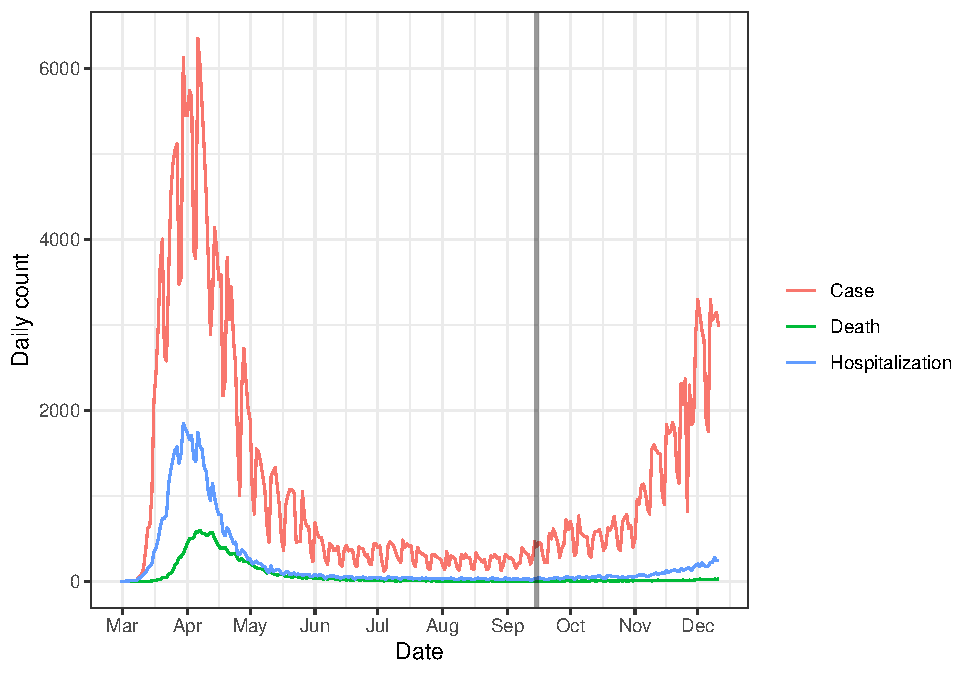
\includegraphics{report_files/figure-latex/unnamed-chunk-3-1.pdf}
\caption{Daily counts of COVID-19 cases, hospitalizations, and deaths in
New York City}
\end{figure}

\hypertarget{task-1}{%
\section{Task 1}\label{task-1}}

Our goal for Task 1.1 was to develop a Newton-Raphson algorithm to fit
Richard curves to each NYC borough's cumulative number of cases for a
pandemic wave. We used a simple gradient descent algorithm that aims to
minimize the sum of squared errors (SSE), \(h(\boldsymbol{\theta})\).

Since \(E[Y_i] = N(t_i, \boldsymbol{\theta})\), then
\(h(\boldsymbol{\theta})\) is defined as:

\[
\begin{aligned}
h(\boldsymbol{\theta}) 
&= \sum_{i=1}^n(Y_i -  N(t_i, \boldsymbol{\theta}))^2 \\
&= \sum_{i=1}^n \left[Y_i - a \left\{1 + d\exp\left\{-k(t_i-t_0)\right\}\right\}^{-1/d}\right]^2
\end{aligned}
\]

The gradient of \(h(\boldsymbol{\theta})\),
\(\nabla h(\boldsymbol{\theta})\), is calculated as:

\[
\begin{aligned}
\nabla h(\boldsymbol{\theta})
 &= -2 \sum_{i=1}^n [Y_i - N(t_i,\boldsymbol{\theta})]\cdot \nabla N(t_i,\boldsymbol{\theta}) \\
 &= -2 \sum_{i=1}^n [Y_i - N(t_i,\boldsymbol{\theta})]\cdot 
 \left(
 \frac{\partial N(t_i,\boldsymbol{\theta})}{\partial a}, 
 \frac{\partial N(t_i,\boldsymbol{\theta})}{\partial k}, 
 \frac{\partial N(t_i,\boldsymbol{\theta})}{\partial d}, 
 \frac{\partial N(t_i,\boldsymbol{\theta})}{\partial t_0}
 \right)^T 
\end{aligned}
\]

where

\[
\begin{aligned}
\frac{\partial N(t_i,\boldsymbol{\theta})}{\partial a} &= \frac{1}{(1 + d e^{-k(t-t_0)})^{1/d}}\\
\frac{\partial N(t_i,\boldsymbol{\theta})}{\partial k} &= \frac{a (t-t_0) e^{-k(t-t_0)}}{(1 + d e^{-k(t-t_0)})^{1+1/d}} \\
\frac{\partial N(t_i,\boldsymbol{\theta})}{\partial d} &= -\frac{a(e^{-k(t-t_0)}d - \text{ln}(1+e^{-k(t-t_0)}d)(1 + e^{-k(t-t_0)}d))}{d^2(1 + d e^{-k(t-t_0)})^{1+1/d}} \\
\frac{\partial N(t_i,\boldsymbol{\theta})}{\partial t_0} &= -\frac{ak e^{-k(t-t_0)}}{(1 + d e^{-k(t-t_0)})^{1+1/d}}
\end{aligned}
\]

Our gradient descent algorithm can be summarized as follows:

\begin{enumerate}
\def\labelenumi{\arabic{enumi}.}
\tightlist
\item
  Set \(\boldsymbol{\theta}_0\), the starting values for
  \(\boldsymbol{\theta}\) (see later in this section for more details on
  how to pick these).
\item
  Update \(\boldsymbol{\theta}\) based on
  \(\boldsymbol{\theta}_{j} = \boldsymbol{\theta}_{j-1} - \lambda \cdot I_{4 \times 4} \nabla h(\boldsymbol{\theta}_{j-1})\),
  where \(\lambda\) is a user-chosen learning rate (setting \(\lambda\)
  is to a small value, such as \(1^{-10}\), works well for this data).
\item
  If \(h(\boldsymbol{\theta}_j) \geq h(\boldsymbol{\theta}_{j-1})\),
  then decrease the learning rate further and recalculate
  \(h(\boldsymbol{\theta}_j)\), replacing \(\lambda\) with
  \(\frac{\lambda}{10}\). Continue repeating this step until
  \(h(\boldsymbol{\theta}_j) < h(\boldsymbol{\theta}_{j-1})\),
  i.e.~until there is a decrease in SSE from the previous iteration.
\item
  Continue repeating steps 3 and 4 until convergence is reached,
  i.e.~when the absolute difference between \(h(\boldsymbol{\theta}_j)\)
  and \(h(\boldsymbol{\theta}_{j-1})\) is smaller than a very small
  tolerance level.
\end{enumerate}

Although our algorithm is not the most efficient algorithm, it has two
main advantages. One, it is simple to compute and does not rely on the
calculation of the Hessian, which is complicated. Two, using the
symmetric and positive definite matrix \(I_{4 \times 4}\) as a
replacement for the Hessian guarantees that we have a descent direction.
This means that we will be able to find some \(\lambda \in (0, 1)\) that
ensures that the updated \(\boldsymbol{\theta}_j\) has a smaller SSE
than the previous iteration's \(\boldsymbol{\theta}_{j-1}\).

In step 1 of the algorithm, the user is required to choose the starting
values, \(\boldsymbol{\theta}_0\). We found that poor choices of
\(\boldsymbol{\theta}_0\) resulted in non-convergence or incorrect
convergence issues. Choices of \(\boldsymbol{\theta}_0\) based on the
observed cumulative cases for the borough and the epidemiological
interpretations of the Richard growth parameters resulted in fast
convergence and good final estimates of \(Y_i\). Our guidelines for how
to tailor the starting values for each borough and wave are as follows:

\begin{itemize}
\item
  Since \(a\) is the upper bound of the Richard growth function, then
  let its starting value be the maximum number of cumulative cases in
  the pandemic wave. For the first wave, this is easily calculated as
  \(\mbox{max}(Y_i)\). For the second wave, since we only have observed
  data for the first half of the wave (i.e.~up until about the
  inflection point), we must estimate what the maximum number of
  cumulative cases will be. We recommend using about
  \(2 \times \mbox{max}(Y_i)\) under the assumption that half of the
  maximum cumulative cases occurs at the inflection point. We made this
  assumption because we saw this trend across the boroughs in the first
  wave and assumed that the second wave would follow a similar pattern.
\item
  Since \(t_0\) is the time of inflection, then let its starting value
  be the time \(t_i\) where the inflection point occurs. This can be
  chosen as the point where the curve goes from convex to concave based
  on a plot of \(Y_i\) against \(t_i\). Note that for the second wave,
  since we only have observed data for the first half of the wave, this
  point will occur towards the end of the observed data.
\item
  Since \(k\) is the growth rate that controls the slope at the
  inflection point, then let its starting value be calculated as the
  slope at the inflection point \(t_0\) standardized by the cumulative
  cases at the inflection point:
  \(\frac{(Y_{i,t_0 + m} - Y_{i,t_0 - m})/[(t_0 + m) - (t_0 - m)]}{Y_{i,t_0}}\),
  where \(Y_{i,t_0 - m}\) and \(Y_{i,t_0 + m}\) are the cumulative cases
  corresponding to \(m\) days before and after the inflection point,
  respectively, \(Y_{i,t_0}\) is the cumulative cases corresponding to
  the inflection point, and \((t_0 + m) - (t_0 - m)\) is a small range
  around the inflection point. This can easily be computed by using two
  points around the inflection point to fit a linear regression,
  regressing \(Y_i\) on \(t_i\).
\item
  Since \(d\) has no epidemiological interpretation, picking its
  starting value is tricky. We found that values between 0 and 0.5
  worked well. However, we advise investigators to try a few different
  values for \(d\) and pick what works best.
\end{itemize}

Figure 2 gives an example of how a starting curve for Wave 1 data on NYC
would look, compared to the final fitted curve. We can see that the
starting curve follows the general trend of the observed cumulative
cases, but the final curve obtained from running our algorithm fits the
observed data much better. We also note that from about \(t_i = 100\) to
\(t_i = 200\) of the first wave, the observed cumulative cases follow a
linear trend, so we would expect that our final Richard growth curve
will never be able to fit the observed data very well in this portion of
the wave since the Richard growth function assumes a sigmoidal shape.

The algorithm described in this section was also used in Task 1.2 to fit
Richard curves to each NYC borough's cumulative number of
hospitalizations and deaths for each pandemic wave.

\begin{figure}
\centering
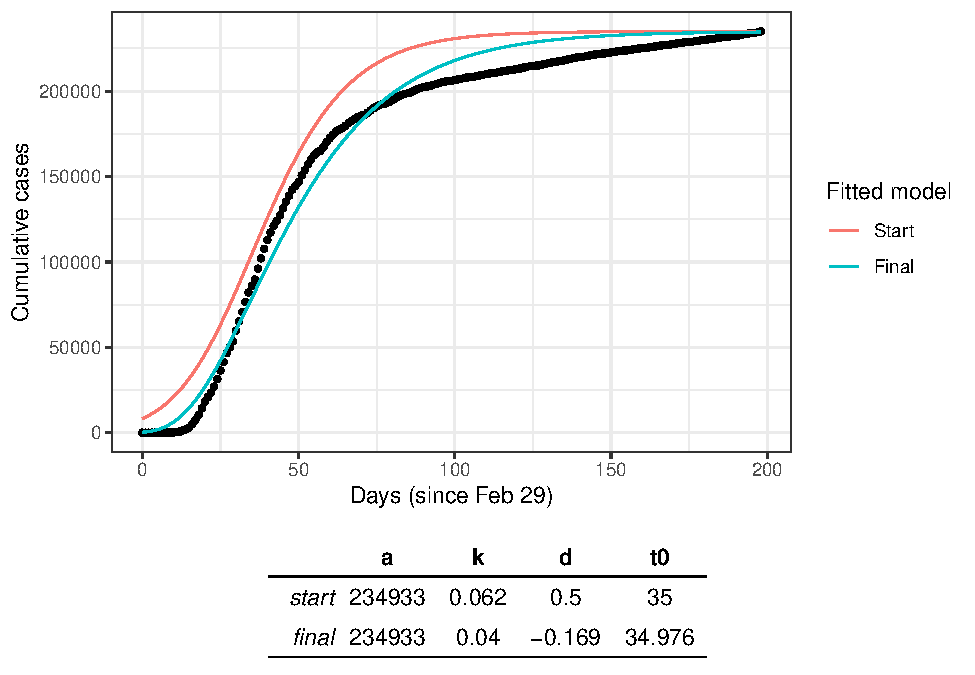
\includegraphics{report_files/figure-latex/unnamed-chunk-5-1.pdf}
\caption{Example for Wave 1 NYC data comparing starting values and
starting curve to the final values and fitted curve obtained from our
algorithm.}
\end{figure}

\hypertarget{task-2}{%
\section{Task 2}\label{task-2}}

\hypertarget{cumulative-cases}{%
\subsection{Cumulative Cases}\label{cumulative-cases}}

We first present the results for cumulative cases in all boroughs to
investigate the algorithm performance. The two COVID-19 waves are
defined as follows: waves 1: February 29, 2020 to September 14, 2020;
wave 2: September 14, 2020 to December 11, 2020.

As discussed in the previous section, the starting values are chosen
based on the following guidelines:

\begin{itemize}
\tightlist
\item
  \(a = \text{max}(Y_i)\);
\item
  \(t_o \approx \text{argmax}(Y_i)\);
\item
  \(k\) is the standardized slope for cumulative cases 4 days before and
  after inflection date.
\item
  \(d\) is 0.5
\end{itemize}

In the first figure, we present the fitted curves (red) and compare the
true cumulative cases (black). From a direct observation, we conclude
that the algorithm performed well in approximating the real data.

\begin{figure}
\centering
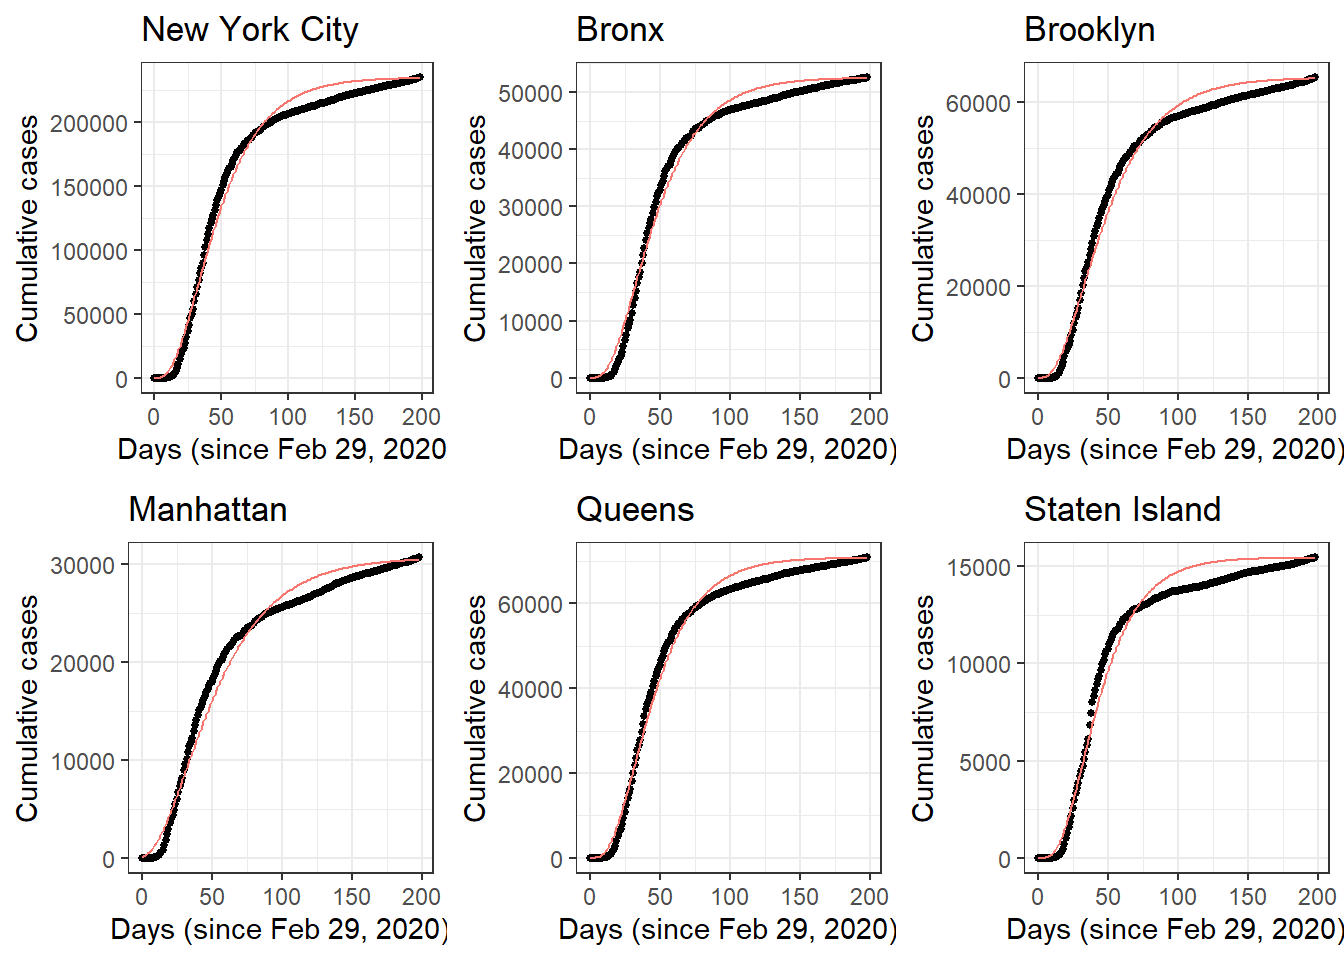
\includegraphics[width=4.16667in,height=\textheight]{plots/case_plots/no_start_curve/wave1_all.png}
\caption{Fitted curves of cumulative cases for first wave}
\end{figure}

We further present the estimates parameters for the first wave
cumulative cases. Since we have access to the first wave data, the
estimated parameters can serve as a validation for the algorithm
performance. By a direction observation of estimated \(a,t_0\)
parameters, we conclude our algorithm performed well since the estimated
parameters approached the truth well.

\begin{figure}
\centering
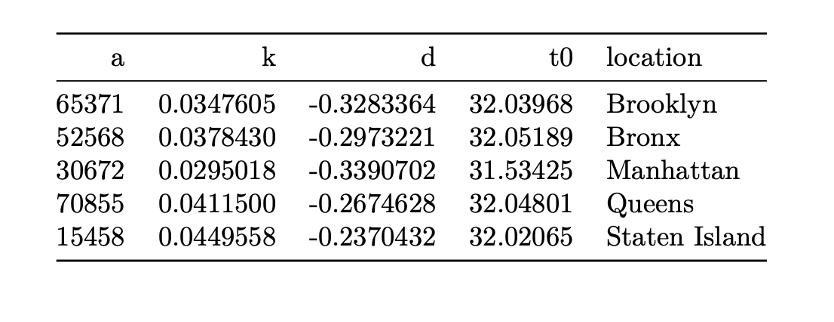
\includegraphics[width=4.16667in,height=\textheight]{plots/case_plots/no_start_curve/wave_1_para.png}
\caption{Estimated parameters of cumulative cases for first wave}
\end{figure}

We then present the fitted curves and estimated parameters for the
second wave cumulative cases. Since we only obtained partial data for
second wave, several assumptions about starting values are made for the
estimation.

\begin{itemize}
\tightlist
\item
  We first assume the inflection point \(t_0\) is at around the end of
  the observed data
\item
  \(a = 2*y_{t0}\) with the assumption that the maximum number of
  cumulative cases will be two times the case number at the inflection
  point
\item
  \(k\) is the standardized slope for cumulative cases 4 days before and
  after inflection date.
\item
  \(d\) is 0.5
\end{itemize}

From the blow figure and estimated parameters, we notice a good recovery
of the true cases cruves with our estimated curves in all boroughs.

\begin{figure}
\centering
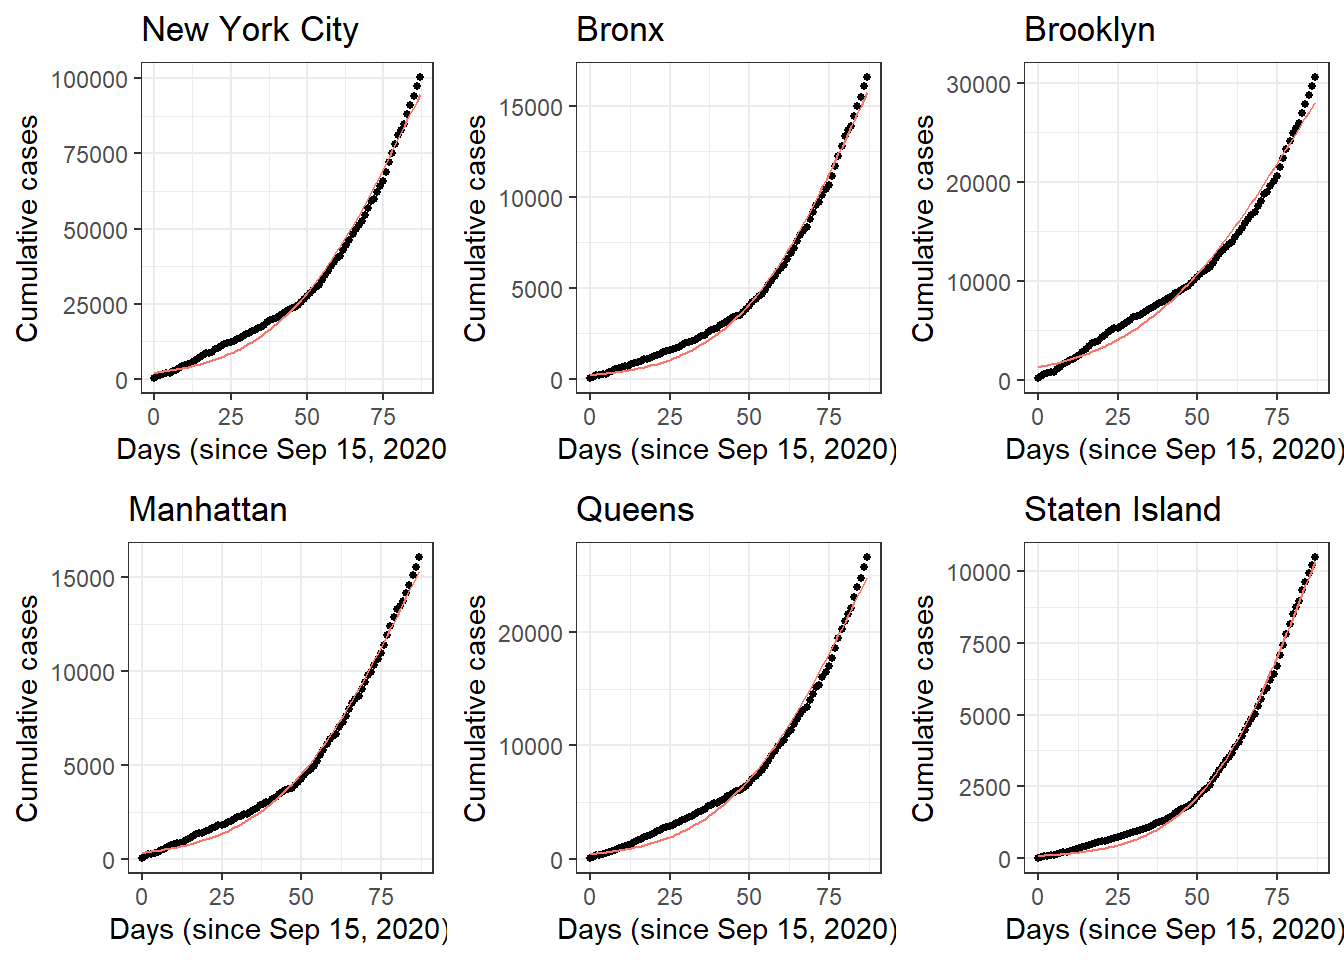
\includegraphics[width=4.16667in,height=\textheight]{plots/case_plots/no_start_curve/wave2_all.png}
\caption{Fitted curves of cumulative cases for second wave}
\end{figure}

\begin{figure}
\centering
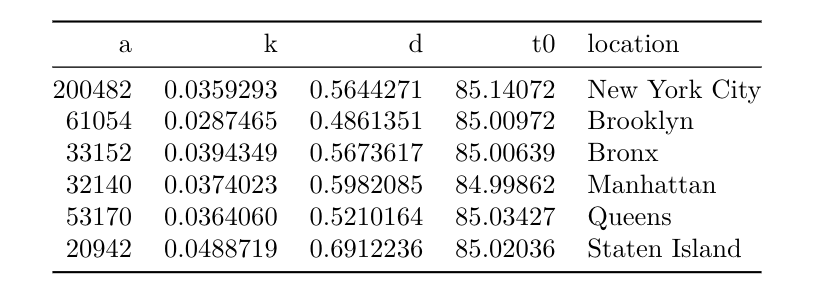
\includegraphics[width=4.16667in,height=\textheight]{plots/case_plots/predictive/case_final_parameters.png}
\caption{Estimated parameters of cumulative cases for second wave}
\end{figure}

\hypertarget{cumulative-hospitalizations}{%
\subsection{Cumulative
Hospitalizations}\label{cumulative-hospitalizations}}

We fit the Richard's growth curve for cumulative hospitalizations in all
boroughs in NYC. Similar to case observations, we split hospitalizations
into two waves: 1) February 29, 2020 to September 14, 2020; 2) September
14, 2020 to December 11, 2020.

When fitting the first wave of hospitalizations, we use the following
assumptions to pick starting values:

\begin{itemize}
\tightlist
\item
  \(a\) is \(\mbox{max}(Hospitalizations)\) for all boroughs and NYC,
  assuming there is not much increase in hospitalization counts or
  health resources to accommodate patients after the curve levels out.
\item
  Different inflection date \(t_0\) for different locations, as we
  observe slopes at different dates fit observations better. There are
  minor differences among inflection dates. Brooklyn and Manhattan have
  March 31 as starting value for inflection date; Staten Island has
  April 1; Queens, Bronx, and NYC have April 3, 2020.
\item
  \(k\) is the standardized slope for cumulative hospitalization data on
  4 days before and after inflection date.
\item
  \(d\) is 0.5
\end{itemize}

Figure 7 are plots for fitted curve for the first hospitalization wave.
Figure 8 are the parameters used to fit the first wave.

\begin{figure}
\centering
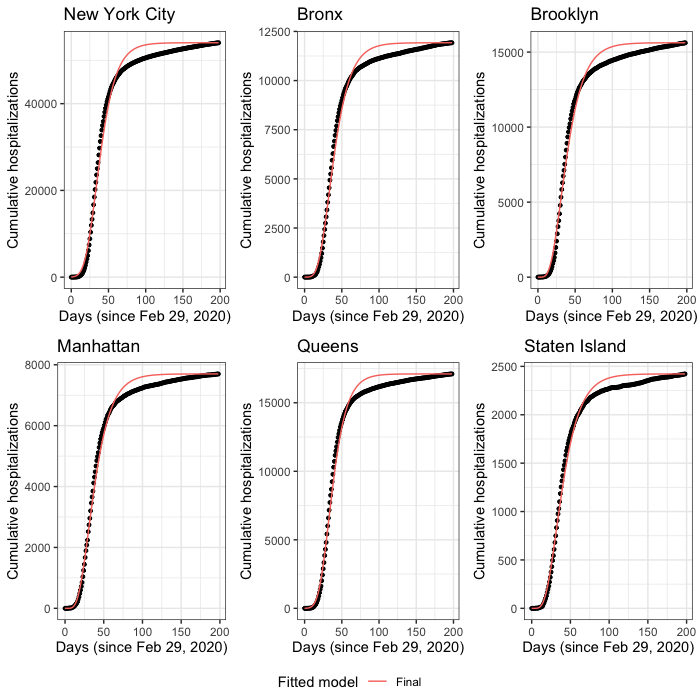
\includegraphics[width=4.16667in,height=\textheight]{plots/hosp_plots/no_start_curve/hosp_wave1_all.png}
\caption{The first hospitalization wave - fitted curves}
\end{figure}

\begin{figure}
\centering
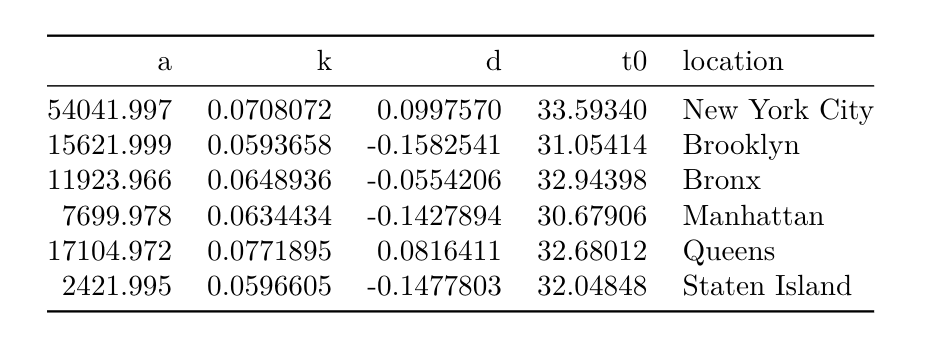
\includegraphics[width=4.16667in,height=\textheight]{plots/hosp_plots/no_start_curve/hosp_wave1_final_parameters.png}
\caption{The first hospitalization wave - parameters}
\end{figure}

The fit is very close to the observations in all locations. The fitted
curve is overestimating hospitalizations around the dates that the curve
starts to level out. However, since healthcare resources were extremely
limited during the outbreak of the pandemic, it is safe to overestimate
than underestimate hospitalization counts. The final fitted \(t_0\) for
all locations are indeed a couple of days apart, corresponding to our
initial belief.

Observed hospitalization in the second wave seems to be the first half
of a regular Richard's growth curve. We do see a gradual increase and
then more rapid increase in hospitalization during this period of time.
The changes in slopes are tricky to model this time. For the second wave
of hospitalization, the initial values are decided as the following:

\begin{itemize}
\tightlist
\item
  \(a\) is \(2.2 \times \mbox{max}(hospitalization)\) for all boroughs
  and NYC, assuming that half of the maximum hospitalization occurs at
  the inflection point.
\item
  December 9, 2020 as \(t_0\) for all locations.
\item
  \(k\) is the standardized slope for cumulative hospitalization data on
  2 days before and after inflection date due to rapid change in
  hospitalizations around our assumed inflection date.
\item
  \(d\) is 0.25 for Staten Island and 0.5 for all other locations.
\end{itemize}

Figure 9 are plots for fitted curve for the second hospitalization wave.
Figure 10 are the parameters used to fit the second wave.

\begin{figure}
\centering
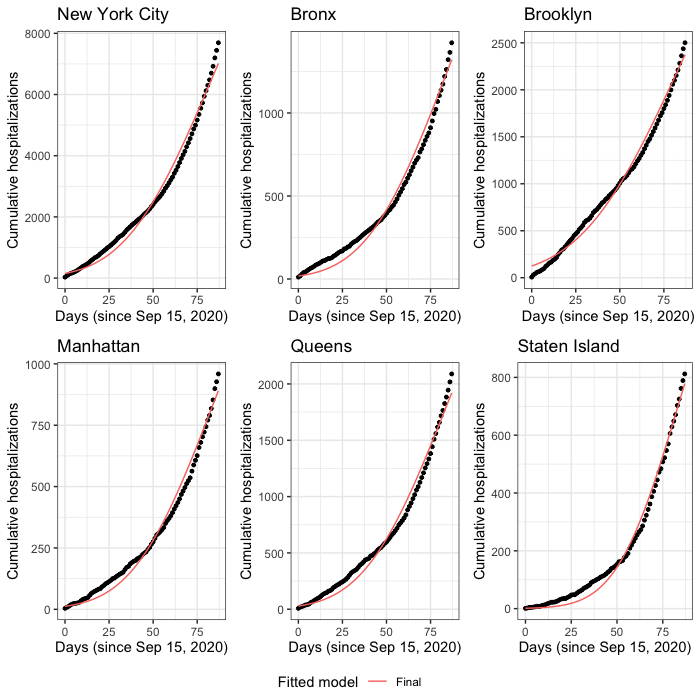
\includegraphics[width=3.125in,height=\textheight]{plots/hosp_plots/no_start_curve/hosp_wave2_all.png}
\caption{The second hospitalization wave - fitted curves}
\end{figure}

\begin{figure}
\centering
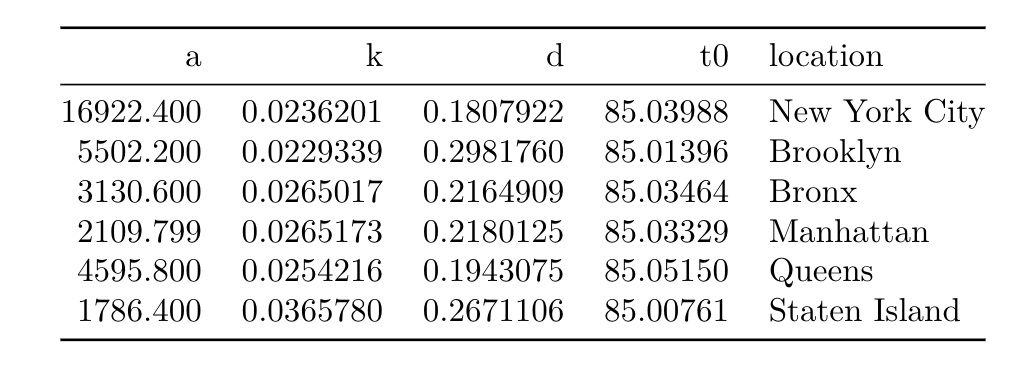
\includegraphics[width=4.16667in,height=\textheight]{plots/hosp_plots/predictive/hosp_final_parameters.png}
\caption{The second hospitalization wave - parameters}
\end{figure}

The fitted curves still look very close to the observation. We tend to
underestimate when the observed hospitalization is mildly increasing,
and overestimate when the speed of the observed increase is growing. The
estimate values for growth rate parameter \(k\) reflect how different
the slope changes in each borough.

\hypertarget{cumulative-deaths}{%
\subsection{Cumulative Deaths}\label{cumulative-deaths}}

We also fit growth curves to estimate cumulative deaths in NYC. We split
the deaths into two waves, in the same way as mentioned previously.

We use the following assumptions to pick starting values:

\begin{itemize}
\tightlist
\item
  \(a\) is \(\mbox{max}(Deaths)\) for all boroughs and NYC.
\item
  All locations have the same starting value \(t_0\), which is April 10,
  2020. This inflection point is later than the ones assumed for cases
  and hospitalizations, as we assume that a rise in deaths will trail
  several days behind rises in cases and hospitalizations.
\item
  \(k\) is the standardized slope for cumulative deaths data on 4 days
  before and after inflection date.
\item
  \(d\) is 0.5.
\end{itemize}

Figure 11 shows plots for fitted death curves for the first wave. Figure
12 shows the final parameters used to fit the first wave curves.

\begin{figure}
\centering
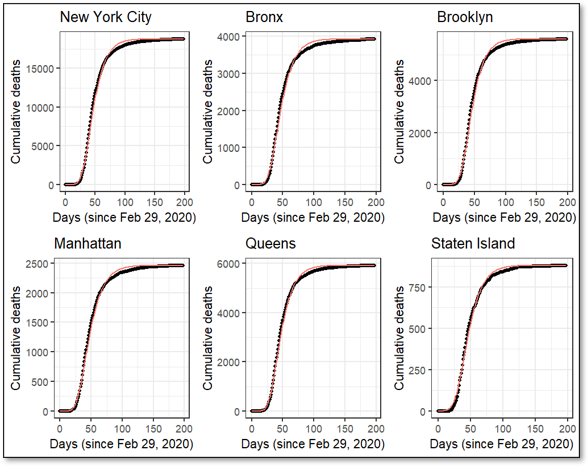
\includegraphics[width=4.16667in,height=\textheight]{plots/death_plots/wave1_plots.png}
\caption{The first death wave - fitted curves}
\end{figure}

\begin{figure}
\centering
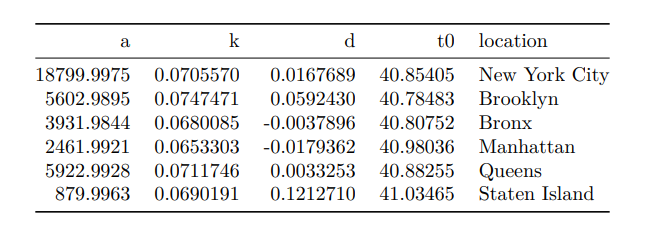
\includegraphics[width=4.16667in,height=\textheight]{plots/death_plots/death_table_1.png}
\caption{The first death wave - parameters}
\end{figure}

The estimated Richard's curve fits the observed deaths curve very well
for each borough. is very close to the observations in all locations.

For the second wave of deaths, the initial values are decided as the
following:

\begin{itemize}
\tightlist
\item
  \(a\) is \(2 \times \mbox{max}(Deaths)\) for all boroughs and NYC,
  assuming that half of the maximum deaths occur at the inflection
  point.
\item
  December 9, 2020 as \(t_0\) for all locations. We would assume that
  the inflection point would be later for deaths than it is for cases
  and hospitalizations, but since we only have data until December 11,
  it did not make sense to try to push the starting inflection date
  further.
\item
  \(k\) is the standardized slope for cumulative deaths data on 2 days
  before and after the inflection date.
\item
  \(d\) is 0.25 for Staten Island and 0.5 for all other locations.
\end{itemize}

Figure 13 are plots for fitted curve for the second death wave. Figure
14 shows the final parameters used to fit the second wave.

\begin{figure}
\centering
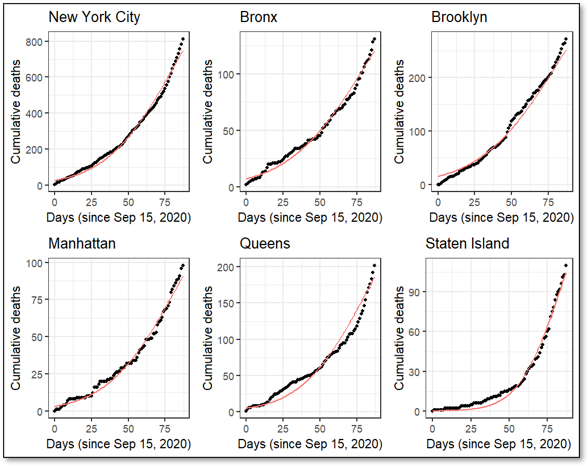
\includegraphics[width=4.16667in,height=\textheight]{plots/death_plots/wave2_plots.png}
\caption{The second death wave - fitted curves}
\end{figure}

\begin{figure}
\centering
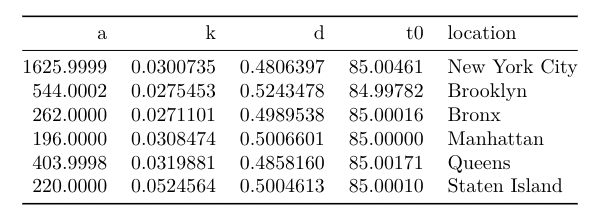
\includegraphics[width=4.16667in,height=\textheight]{plots/death_plots/deaths_final_prarameters.png}
\caption{The second death wave - parameters}
\end{figure}

The fitted curves look relatively close to the observed death trends.
The shapes of the curves across boroughs seem very different, showing
that the predicted trends in deaths by the end of the second wave will
vary across boroughs.

\hypertarget{task-3}{%
\section{Task 3}\label{task-3}}

\hypertarget{cumulative-cases-1}{%
\subsection{Cumulative Cases}\label{cumulative-cases-1}}

From the previous task, we successfully estimated and obtained
parameters that approximated the first half of the second wave data
well. A natural extrapolation would be extending the curves so that we
may predict the cumulative cases based on th observed the data. Hence,
we utilize the estimated final parameters and use that for cumulative
cases prediction.

We incorporate borough population to infer cases per 100,000 capita so
that based on the y axis we are able to make a direct comparison of the
severity of the second wave. Based on the interpretation of the
estimated parameters, we obtained the following observations:

\begin{itemize}
\tightlist
\item
  \(a\) can be interpreted as maximum number of cumulative cases in each
  borough. Staten Island is predicted to have the largest cases per
  100,000 capita and Manhattan is predicted to have the smallest
\item
  \(k\) can be interpreted as standardized slope at the inflection
  point. It Provides intuition of the rate of cases increase at
  inflection point. Staten Island has biggest \(k\) while Brooklyn has
  smallest \(k\).
\end{itemize}

Therefore, based on the previous prediction and observation, we would
suggestion that distributing vaccination to the boroughs with higher
predicted cumulative cases per capita and large rate of cases increase.
In this case, Staten Island should be prioritized for vaccination
rollout.

\begin{figure}
\centering
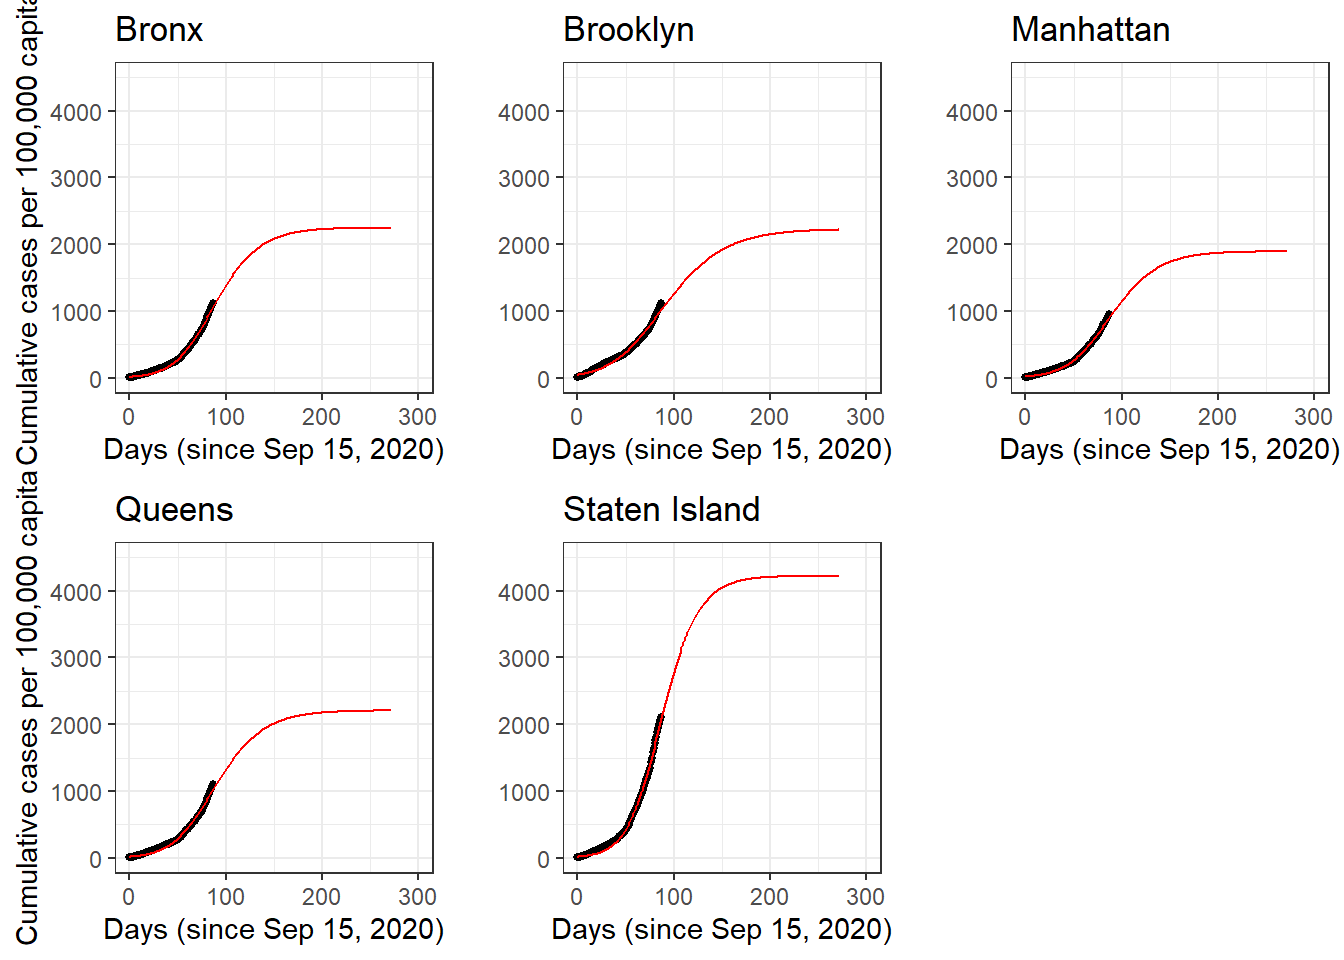
\includegraphics[width=3.125in,height=\textheight]{plots/case_plots/predictive/all_pred.png}
\caption{Predicted cases for each borough}
\end{figure}

\begin{figure}
\centering
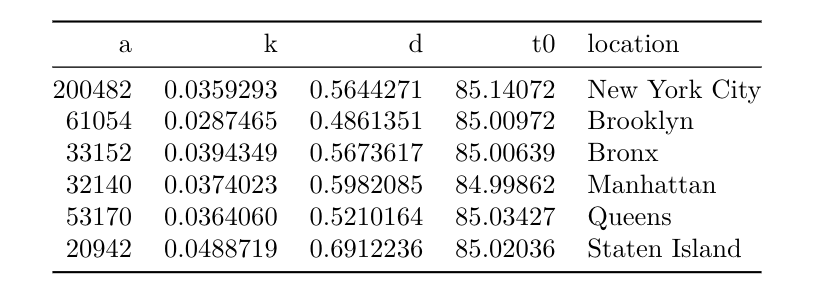
\includegraphics[width=3.125in,height=\textheight]{plots/case_plots/predictive/case_final_parameters.png}
\caption{Estimated parameters of cumulative cases for second wave}
\end{figure}

\hypertarget{cumulative-hospitalizations-1}{%
\subsection{Cumulative
Hospitalizations}\label{cumulative-hospitalizations-1}}

We used the parameters in the fit for second wave of cumulative
hospitalizations to make long-term predictions and hope to draw insight
on vaccine distribution from the predicted curve.

\begin{figure}
\centering
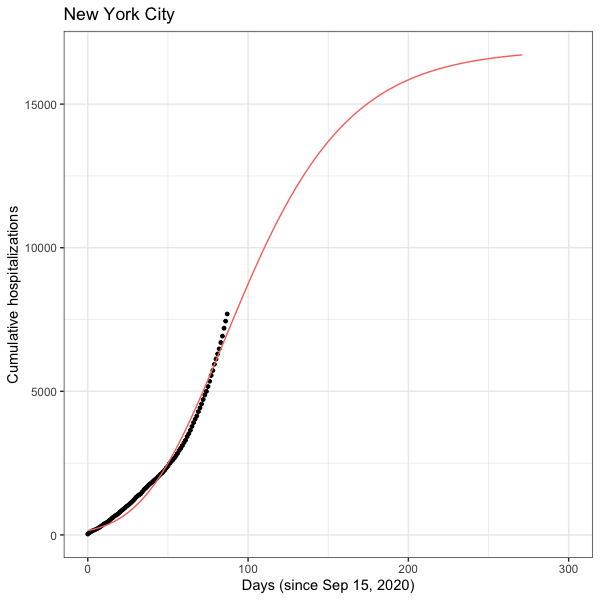
\includegraphics[width=4.16667in,height=\textheight]{plots/hosp_plots/predictive/hosp_nyc_pred.png}
\caption{Predicted hospitalization for NYC}
\end{figure}

To make our predictions more comparable, we plotted predicted cumulative
hospitalizations per 100,000 capita for each borough.

\begin{figure}
\centering
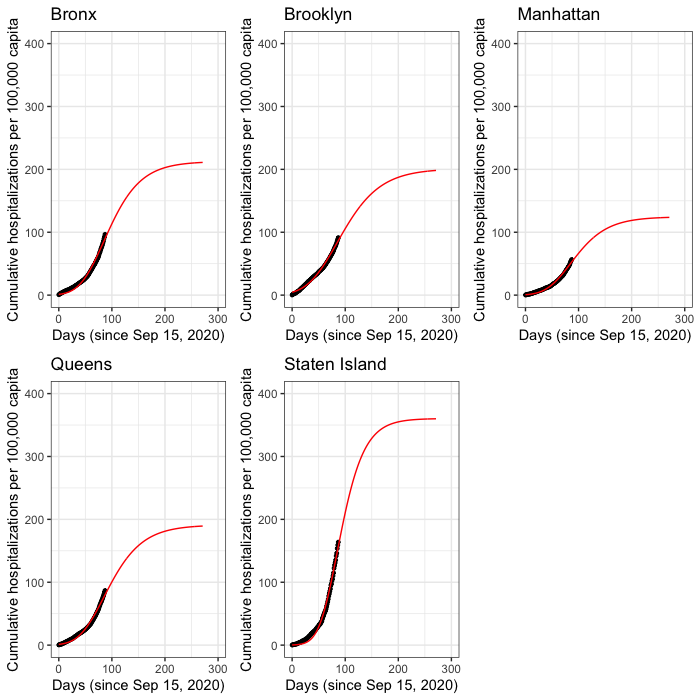
\includegraphics[width=4.16667in,height=\textheight]{plots/hosp_plots/predictive/hosp_all_pred.png}
\caption{Predicted hospitalization for each borough}
\end{figure}

Unfortunately, Staten Island has the highest predicted cumulative
hospitalizations per 100,000 capita and its predicted growth rate is the
highest.

Bronx and Manhattan both have the second highest predicted growth rate.
But Bronx has the higher predicted hospitalizations per 100,000 capita.

Even though growth rate and predicted hospitalization per 100,000 capita
are different for each borough, the predicted inflection date is almost
the same for all boroughs. \(t_0 = 85\) corresponds to December 9, 2020.
This date is also very similar to the predicted inflection date for
cumulative cases. This could be a result of rapid disease progression,
as some people who were contracted need to be hospitalized immediately.

COVID-19 vaccines first became available in the US on December 14, 2020
according to U.S. Department of Health \& Human Services. Therefore,
while prioritizing hot spots such as Staten Island and Bronx, the
government should also prepare enough inventory to meet needs city-wide
to provide maximum protection against COVID-19 due to its rapid disease
progression.

\hypertarget{cumulative-deaths-1}{%
\subsection{Cumulative Deaths}\label{cumulative-deaths-1}}

The predicted plots for cumulative deaths in the second wave, scaled for
population size, for each borough are shown below in Figure 19.

\begin{figure}
\centering
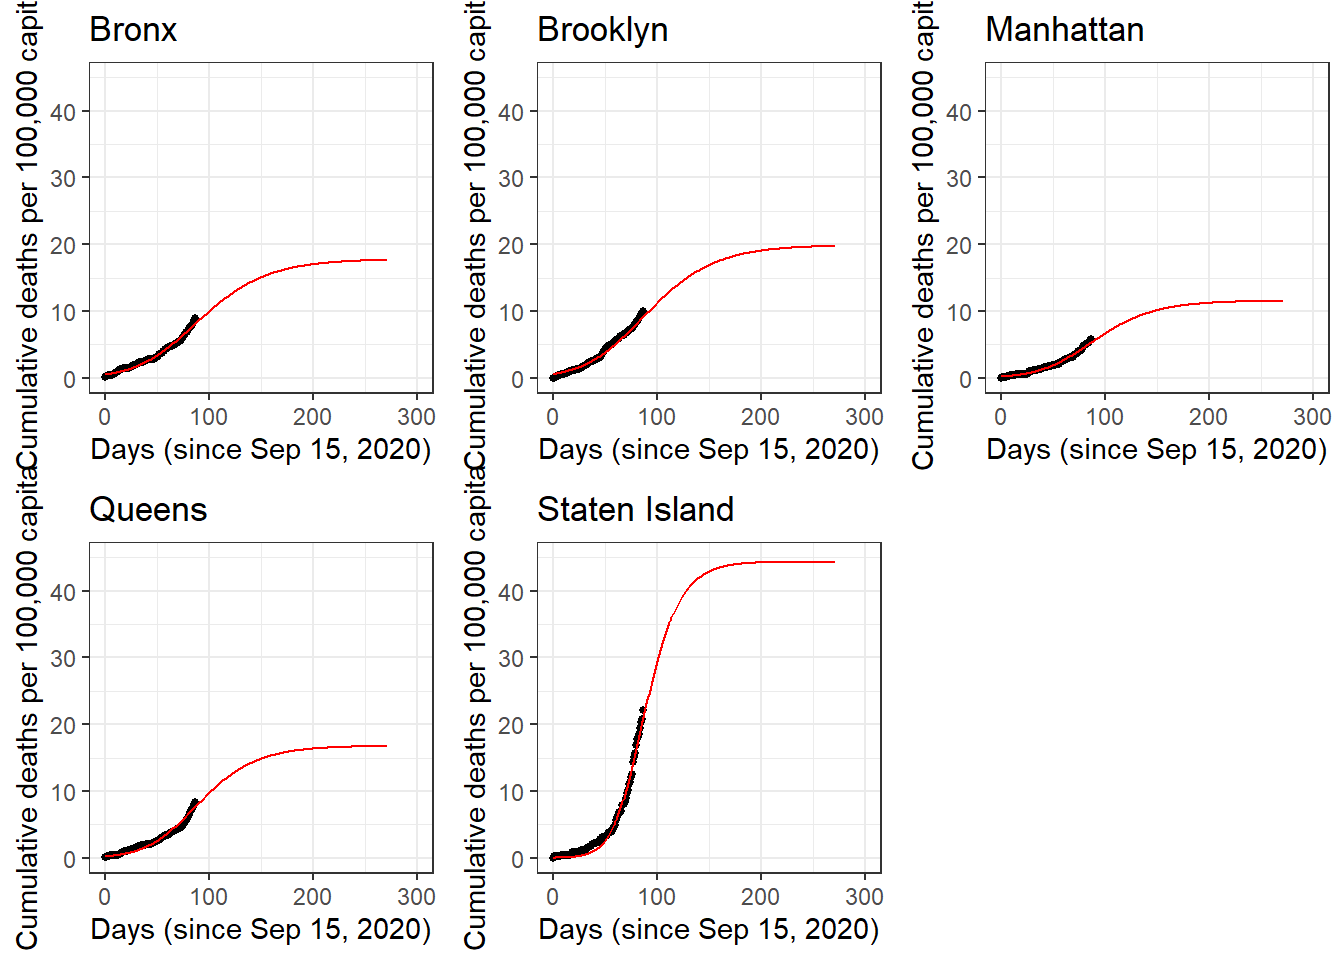
\includegraphics[width=4.16667in,height=\textheight]{plots/death_plots/predictive/all_pred.png}
\caption{Predicted hospitalization for NYC}
\end{figure}

Based on the final parameters shown in Figure 14, we see that Brooklyn
and Manhattan have the highest estimated k values (slope at the
inflection point). Brooklyn and Queens have the highest number of
estimated cumulative deaths. Staten Island is consistently predicted to
increase quickly and have a high rate of deaths overall.

When we scale for population in the plots in the figure above, we see
that Brooklyn and the Bronx actually have the highest number of
predicted cumulative deaths per 100,000 capita.

Interestingly, in Brooklyn and the Bronx, cases aren't expected to
increase at a quick rate, but hospitalizations and deaths are. This
would give us motivation us to roll out vaccinations quickly to Brooklyn
and the Bronx, to prevent severe cases and therefore hospitalizations
and deaths.

\hypertarget{conclusions}{%
\section{Conclusions}\label{conclusions}}

\emph{Task 1.} Richard's growth curves fit relatively well to COVID-19
case, hospitalization, and death data when starting values were chosen
well and waves were specified appropriately.

\emph{Task 2.} From fitting the curves, we learned that Brooklyn and
Queens had experienced the greatest number of cases, hospitalizations,
and deaths by the end of each wave. Empirically, curves varied more
between boroughs during the second wave than during the first.

\emph{Task 3.} Extending our wave 2 fitted curves and accounting for
each borough's population size allowed us to make recommendations for
vaccine rollout. We recommend that, if the number of vaccines is
limited, that we target Staten Island, which is expected to see the
largest number of cases, deaths, and hospitalizations per capita. We
also suggest rolling out vaccines quickly to Brooklyn and the Bronx,
where the number of hospitalizations and deaths are expected to be large
and to increase at a quick rate around the inflection point. It is
important to target these areas because we noticed that even though the
number of cases may be lower, the large amount of hospitalizations and
deaths tells us that COVID-19 may take a large toll on healthcare
facilities in these areas.

\end{document}
